\documentclass[a4paper, 12pt]{article}

\usepackage[T2A]{fontenc}
\usepackage[utf8]{inputenc}
\usepackage[english,russian]{babel} %локализация
\usepackage{graphicx}%Вставка картинок правильная
\usepackage{float}%"Плавающие" картинки
\usepackage{wrapfig}%Обтекание фигур (таблиц, картинок и прочего)
\usepackage{fancybox,fancyhdr} %колонтитулы
\usepackage{amsmath, amsfonts, amssymb, amsthm, mathtools} %математика
\usepackage[left=1.5cm,right=1.5cm,
    top=1cm,bottom=1.2cm,bindingoffset=0cm]{geometry}
%\usepackage[12pt]{extsizes} % размер шрифта

%\documentclass[a4paper]{article}
\usepackage[14pt]{extsizes}
\usepackage[T2A]{fontenc}
\usepackage[utf8]{inputenc}
\usepackage[russian]{babel}
\usepackage{setspace,amsmath}
\usepackage{graphicx}
\usepackage{epigraph}
\usepackage{csquotes}
\usepackage[unicode, pdftex, hidelinks]{hyperref}
\usepackage{amssymb}
\usepackage{caption}
\usepackage{amsthm}
\usepackage{float}
\usepackage{wrapfig}
\usepackage{multirow}

\newtheorem*{definition}{\sc{Definition}}
\newtheorem*{proposition}{\sc{Proposition}}
\newtheorem*{corollary}{\sc{Corollary}}
\newtheorem*{claim}{\sc{Claim}}
\newtheorem*{properties}{\sc{Properties}}
\newtheorem*{remark}{\sc{Remark}}
\DeclareMathOperator{\N}{\mathbb{N}}
\DeclareMathOperator{\Z}{\mathbb{Z}}
\DeclareMathOperator{\Q}{\mathbb{Q}}
\DeclareMathOperator{\R}{\mathbb{R}}
\RequirePackage{caption}
\DeclareCaptionLabelSeparator{d}{}


%% Перенос знаков в формулах (по Львовскому)
\newcommand*{\hm}[1]{#1\nobreak\discretionary{}
{\hbox{$\mathsurround=0pt #1$}}{}}


\author{Вехов В. В.}

\title{Демон Максвелла\\ (парадокс с храповиком)\\ Вопрос по выбору}

\date{2024}

\begin{document}
\maketitle

\\\
\\\
\center{
\includegraphics[scale=0.2]{logo.png}}
\newpage

\vspace {20 mm}
\textbf{Введение}

В данной работе рассматриваются два схожих парадокса (парадокс с храповиком, является частным случаем парадокса Максвелла), связанных с выполнением второго начала термодинамики.


\newline\

В науке, как и в художественной литературе, встречаются фантастические персонажи. Пожалуй, больше всего их было вымышлено в процессе обсуждения второго начала термодинамики. Самым популярным из них стал демон Максвелла, которого придумал Джеймс Клерк Максвелл, автор знаменитой системы уравнений Максвелла, полностью описывающей электромагнитные поля. Второе начало (или закон) термодинамики имеет множество формулировок, физический смысл которых идентичен: изолированная система не может самопроизвольно переходить из менее упорядоченного состояния в более упорядоченное. Так, газ, состоящий из молекул, движущихся с различными скоростями, не может самопроизвольно разделиться на две части, в одной из которых соберутся молекулы, движущиеся быстрее среднестатистической скорости, а в другой - медленнее.\\

\newline\

\textbf{Суть парадоксов}\\

1) (Демон Максвелла) Представим себе следующий мысленный эксперимент: предположим, сосуд (рис.1) с газом разделён непроницаемой перегородкой на две части: правую и левую. В перегородке есть отверстие с устройством (так называемый демон Максвелла), которое позволяет пролетать быстрым (горячим) молекулам газа только из левой части A сосуда в правую B, а медленным (холодным) молекулам — только из правой части сосуда в левую (демон «открывает» и «закрывает» перегородку перед молекулами, оценивая их скорость). Тогда через большой промежуток времени «горячие» (быстрые) молекулы окажутся в правом сосуде, а «холодные» останутся в левом.

Таким образом, получается, что демон Максвелла позволяет нагреть правую часть сосуда и охладить левую без дополнительного подвода энергии к системе. Энтропия для системы, состоящей из правой и левой части сосуда, в начальном состоянии больше, чем в конечном, что противоречит закону возрастания энтропии (адиабатически изолированной системы).

\begin{figure}[h!]
\center{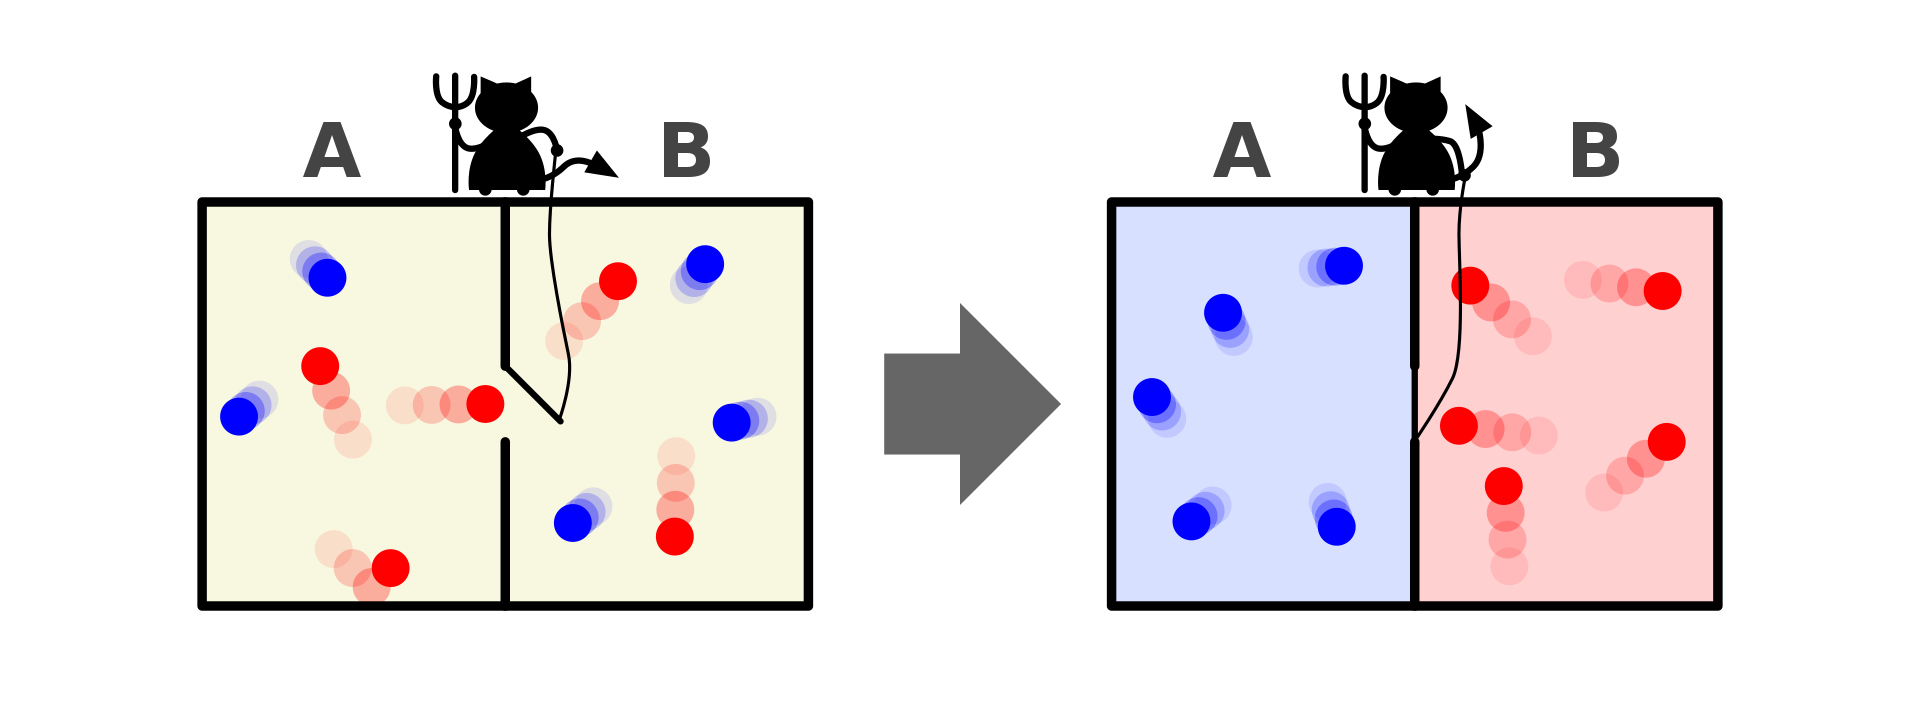
\includegraphics[width=0.70\textwidth]{Maxwell's_demon.svg.png}}
\caption{Демон Максвелла.}
\label{ris:image}
\end{figure}

2) (Машина Фейнмана) Предположим, что в сосуде находится газ при некоторой температуре, а внутри имеется вертушка (рис.2) с температурой $T_1$. На другой стороне оси вертушки расположен храповик с собачкой при температуре $T_2 = T_1 = T$, который может вертеться только в одну сторону. Собачка пресечёт попытки вертушки поворачиваться в одну сторону, а в другую - разрешит. На ось насажен барабан, к которому ниткой привязан небольшой груз.

Колесико должно будет медленно поворачиваться, поднимая груз. Фактически, храповик с собачкой играют роль демона. Таким образом, получается, что машина совершает работу только за счёт охлаждения сосуда, что невозможно.
\begin{figure}[h!]
\center{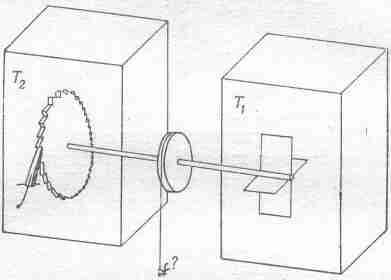
\includegraphics[width=0.41\textwidth]{Машина.jpg}}
\caption{Машина Фейнмана.}
\label{ris:image}
\end{figure}

\newpage
\textbf{Объяснение. Демон Максвелла.}

1) Демон должен воспользоваться каким-либо измерительным прибором для оценки скоростей молекул, например электрическим фонариком. Поэтому надо рассмотреть энтропию системы, состоящей из газа при постоянной температуре $T_0$ демона и фонарика, включающего заряженную батарейку и электрическую лампочку. Батарейка должна нагревать нить лампы фонарика до высокой температуры $T_1 > T_0$ с целью получения квантов света с энергией $\hbar\omega > T_0$  для того, чтобы кванты света распознавались на фоне теплового излучения с температурой $T_0$.

2) Предположим, что демон сумел получить разность температур $\Delta T$:
$T_B$ > $T_A$, $T_B - T_A = \Delta T$, $T_B = T + \frac{1}{2} \Delta T$ и $T_A = T - \frac{1}{2} \Delta T$. Далее демон выбирает быструю молекулу в А с кинетической энергией $\frac{3}{2}kT(1+\varepsilon_1)$ и направляет её в B. Затем выбирает медленную молекулу в B с кинетической энергией  $\frac{3}{2}kT(1-\varepsilon_2)$ и даёт ей проникнуть в A.

3) Для того, чтобы пронаблюдать эти 2 молекулы, демону требуется 2 световых кванта, т.е. увеличение энтропии
\begin{equation}
 \Delta S_d = 2\frac{h\nu}{T_0} = 2kb,
 \label{eq:ref}
\end{equation}
где $b = \frac{h\nu}{kT_0}$ > 1 (необходимое условие получения видимого света).

4) В результате обмена молекулами $\DeltaQ = \frac{3}{2}kT(\varepsilon_1+\varepsilon_2)$ - перенос энергии из А в B. Тогда полная энтропия изменяется на $\Delta S_i = \frac{\Delta Q}{T_B} - \frac{\Delta Q}{T_A} = -\Delta Q \frac{\Delta T}{T^2}$, т.е.
\begin{equation}
 \Delta S_i = -\frac{3}{2}k(\varepsilon_1+\varepsilon_2)\frac{\Delta T}{T}
 \label{eq:ref}
\end{equation}

5) Величины $\varepsilon_1$, $\varepsilon_2$ не велики, $\Delta T \ll T$, поэтому из (1), (2)

$\Delta S = 2kb -\frac{3}{2}k(\varepsilon_1+\varepsilon_2)\frac{\Delta T}{T} > 2k - \frac{3}{2}k = \frac{k}{2} > 0$, т.е. выполняется закон возрастания энтропии и второе начало термодинамики не нарушается.\\

\newpage

\textbf {Объяснение. Машина Фейнмана.}

1) Поскольку после проскока зубца храповика собачка должна вернуться в прежнее положение, то необходима некоторая пружинка. Предположим, что части машины идеально упруги. Когда собачка пройдёт через конец зубца и сработает пружинка, собачка ударится о колесико и начнёт подпрыгивать.

Если в это время произойдёт флуктуация, то вертушка может повернуться в другую сторону, т.к. когда собачка приподнята, зубец может под ней проскользнуть.

Чтобы это избежать, необходимо как-то гасить эти прыжки. При этом гашении энергия собачки перейдёт к храповику - он нагреется. При этом также нагреется и сам газ.

Поскольку при этом собачка и храповик, обладая некоторой температурой, подвержены также и броуновскому движению, поэтому время от времени собачка случайно поднимается и проходит мимо зубца в тот момент, когда броуновское движение вертушки пытается повернуть её назад. Чем горячее предмет, тем чаще это бывает.

2) Таким образом, иногда от щелчков по крыльям вертушки собачка поднимается и вертушка поворачивается, а иногда, когда вертушка стремится повернуть назад, собачка оказывается уже приподнятой (из-за флуктуаций движений этого конца оси) и храповик поворачивает обратно.

3) Чтобы поднять собачку до верха зубца, надо проделать работу $\varepsilon$ против натяжения пружинки. Согласно распределению Больцмана вероятность того, что система накопит достаточно энергии, чтобы поднять собачку до края зубца
\begin{equation}
p = \exp{-\frac{\varepsilon}{kT_1}}.
\label{eq:ref}
\end{equation}

4) Вероятность того, что собачка поднимется случайно равна
\begin{equation}
p = \exp{-\frac{\varepsilon}{kT_2}}.
\label{eq:ref}
\end{equation}

С учётом $T_1 = T_2 = T$ получим, что (3) $\equiv$ (4). Значит, сколько раз собачка случайно поднимется, давая храповику свободно повернуться назад, столько же раз окажется достаточно энергии, чтобы при прижатой собачке вертушка повернулась вперед.

2.5) Получается равновесие, а не вращение. Второе начало термодинамики выполняется.

\newline\

\textbf {Заключение:}

В работе были показаны причины, по которым парадоксы с демоном Максвелла и с храповиком и собачкой Фейнмана не нарушают второе начало термодинамики.

\newline\

\textbf{Литература:}

1) Фейнмановские лекции по физике. Т IV, глава 46 $\S 1-3$;

2) \text{https://ru.wikipedia.org/wiki/ДемонМаксвелла}

3) \text{https://elementy.ru/trefil/21166/DemonMaksvella}


\end{document}
